\documentclass{beamer}

\usepackage[utf8]{inputenc}
\usepackage{amsmath,amssymb,tikz-cd}

\DeclareMathOperator{\im}{im}

\title{Spectral Sequences}
\author{Braden Hoagland}
\institute{Math 502: Algebraic Structures II}
\date{}

\usecolortheme{orchid}

\begin{document}

%--------------------------------------------------------------------------------
% Title Page
%--------------------------------------------------------------------------------

\begin{frame}
	\titlepage
\end{frame}

%--------------------------------------------------------------------------------
% Intro
%--------------------------------------------------------------------------------

\begin{frame}[fragile]
	\frametitle{Homology}

	\begin{itemize}
		\item Chain complex:
	\begin{equation*}
		\begin{tikzcd}
			\cdots\rar{d_{n+2}}&C_{n+1}\rar{d_{n+1}}&C_n\rar{d_n}&C_{n-1}\rar{d_{n-1}}&\cdots
		\end{tikzcd}
	\end{equation*}
	such that $d^{2}=0$.

		\item $n$-th homology: $H_{n}(A) = \ker d_n / \im d_{n+1}$.
	\end{itemize}
\end{frame}

%--------------------------------------------------------------------------------
% Preliminaries
%--------------------------------------------------------------------------------

\begin{frame}[fragile]
	\frametitle{Preliminaries}

	\setbeamercolor{block title}{use=structure,fg=white,bg=green!75!black}
	\begin{theorem}
		A homomorphism of complexes induces a homomorphism of homologies.
	\end{theorem}
	\[
	\begin{tikzcd}
		\cdots \rar & A_{n+1} \dar{f_{n+1}}\arrow[r] & A_n \arrow[r]\arrow[d,"f_n"] & A_{n-1} \arrow[r] \arrow[d,"f_{n-1}"]& \cdots \\
		\cdots \rar & B_{n+1} \arrow[r] & B_n \arrow[r] & B_{n-1} \arrow[r] & \cdots
	\end{tikzcd}
	\]
\end{frame}

\begin{frame}[fragile]
	\frametitle{Preliminaries}

	\setbeamercolor{block title}{use=structure,fg=white,bg=green!75!black}
        \begin{theorem}
                A homomorphism of complexes induces a homomorphism of homologies.
        \end{theorem}
	\[
        \begin{tikzcd}
		\cdots \rar & H_{n+1}(A) \dar\arrow[r] & H_{n}(A) \arrow[r]\arrow[d] & H_{n-1}(A) \arrow[r] \arrow[d]& \cdots \\
		\cdots \rar & H_{n+1}(B) \arrow[r] & H_n(B) \arrow[r] & H_{n-1}(B) \arrow[r] & \cdots
        \end{tikzcd}
        \]
\end{frame}

\begin{frame}[fragile]
	The homomorphism of homologies is given by
	\begin{align*}
		\phi_{n}:H_n(A)&\to H_n(B)\\
		[a]&\mapsto [f_n(a)].
	\end{align*}
	Can check it's well-defined (sends kernels to kernels and images to images) with a diagram chase.
\end{frame}

\begin{frame}
	\frametitle{Preliminaries}

	\setbeamercolor{block title}{use=structure,fg=white,bg=green!75!black}
	\begin{theorem}
	Suppose $0\to A\to B\to C\to 0$ is a short exact sequence of complexes, then there is a long exact sequence of homologies
	\[
        \cdots \to H_{n}(A)\to H_{n}(B) \to H_{n}(C) \to H_{n-1}(A) \to H_{n-1}(B) \to  \cdots.
	\]
	\end{theorem}
\end{frame}


%--------------------------------------------------------------------------------
% Filtered Complexes
%--------------------------------------------------------------------------------

\begin{frame}
	\frametitle{Filtered Complexes}

	\begin{itemize}
		\item Now for the main problem: suppose we want to calculate the homology of a \textit{filtered complex}.
		\item We can build our complex as a sequence of subcomplexes.
	\end{itemize}
\end{frame}

\begin{frame}
	\frametitle{Filtered Complexes}

	\[
		\cdots \;\subset\; F_{p-1}C \;\subset\; F_{p}C \;\subset\; F_{p+1}C \;\subset\; \cdots
	\] 
	\vspace{5mm}
	\begin{figure}[H]
		\centering
		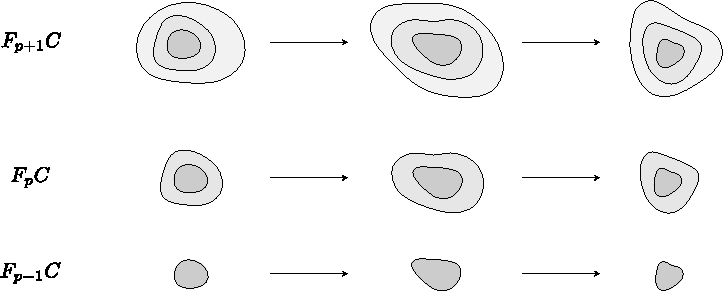
\includegraphics[scale=0.8]{fig/filtered-complex.pdf}
	\end{figure}
\end{frame}

\begin{frame}[fragile]
	\frametitle{Filtered Complexes}

	Induces a bigrading on the complex.
	\begin{overprint}
		\onslide<1>
		\[
		\begin{tikzcd}
			F_{p+1}C_{n+1}&F_{p+1}C_{n}&F_{p+1}C_{n-1}\\
			F_{p}C_{n+1}&F_{p}C_{n}&F_{p}C_{n-1}\\
			F_{p-1}C_{n+1}&F_{p-1}C_{n}&F_{p-1}C_{n-1}
		\end{tikzcd}
		\] 

		\onslide<2>
		\[
		\begin{tikzcd}
			F_{p+1}C_{n+1}\arrow[r]\arrow[dr]\arrow[ddr]&F_{p+1}C_{n}&F_{p+1}C_{n-1}\\
			F_{p}C_{n+1}&F_{p}C_{n}\rar\arrow[dr]&F_{p}C_{n-1}\\
			F_{p-1}C_{n+1}&F_{p-1}C_{n}&F_{p-1}C_{n-1}
		\end{tikzcd}
		\] 
	\end{overprint}
	\vfill

	\onslide<2> Filtered complex: $d(F_{p}C_{n}) \subset F_{p}C_{n-1}$.
	\vspace{5mm}

	\onslide<2> $F$ is \textit{bounded} if it has a finite number of levels.
\end{frame}

\begin{frame}
	\frametitle{Calculating Homology}

	\begin{itemize}
		\item Suppose calculating $H_{*}(C)$ directly is diffiult.
		\item  We can try a ``divide and conquer" strategy to make the computation easier.
	\end{itemize}
\end{frame}

\begin{frame}[fragile]
	\frametitle{Calculating Homology}

	Idea 1: Calculate the homology row by row, then sum them.
	\[
        \begin{tikzcd}
                F_{p+1}C_{n+1}\rar&F_{p+1}C_{n}\rar&F_{p+1}C_{n-1}\\
                F_{p}C_{n+1}\rar&F_{p}C_{n}\rar&F_{p}C_{n-1}\\
                F_{p-1}C_{n+1}\rar&F_{p-1}C_{n}\rar&F_{p-1}C_{n-1}
        \end{tikzcd}
        \]
	\onslide<2> Fails because each row is a subset of the rows above it.
\end{frame}

\begin{frame}[fragile]
	\frametitle{Calculating Homology}

	Idea 2: Quotient each row by the rows below it, then calculate homology row by row and sum them.
	\[
	\begin{tikzcd}
		\frac{F_{p+1}C_{n+1}}{F_{p}C_{n+1}}\rar&\frac{F_{p+1}C_{n}}{F_{p}C_{n}}\rar&\frac{F_{p+1}C_{n-1}}{F_{p}C_{n-1}}\\
		\frac{F_{p}C_{n+1}}{F_{p-1}C_{n+1}}\rar&\frac{F_{p}C_{n}}{F_{p-1}C_{n}}\rar&\frac{F_{p}C_{n-1}}{F_{p-1}C_{n-1}}\\
		\frac{F_{p-1}C_{n+1}}{F_{p-2}C_{n+1}}\rar&\frac{F_{p-1}C_{n}}{F_{p-2}C_{n}}\rar&\frac{F_{p-1}C_{n-1}}{F_{p-2}C_{n-1}}
        \end{tikzcd}
	\] 
	{\color{white}Still fails. The rows aren't subsets of each other anymore, but $d$ still travels between rows.}
\end{frame}

\begin{frame}[fragile]
	\frametitle{Calculating Homology}

	Idea 2: Quotient each row by the rows below it, then calculate homology row by row and sum them.
	\[
		\begin{tikzcd}
			\frac{F_{p+1}C_{n+1}}{F_{p}C_{n+1}}\rar\arrow[rd,dashed]\arrow[rdd,dashed]&\frac{F_{p+1}C_{n}}{F_{p}C_{n}}&\frac{F_{p+1}C_{n-1}}{F_{p}C_{n-1}}\\
			\frac{F_{p}C_{n+1}}{F_{p-1}C_{n+1}}&\frac{F_{p}C_{n}}{F_{p-1}C_{n}}\rar\arrow[rd,dashed]&\frac{F_{p}C_{n-1}}{F_{p-1}C_{n-1}}\\
			\frac{F_{p-1}C_{n+1}}{F_{p-2}C_{n+1}}&\frac{F_{p-1}C_{n}}{F_{p-2}C_{n}}&\frac{F_{p-1}C_{n-1}}{F_{p-2}C_{n-1}}
		\end{tikzcd}
        \]

	Still fails. The rows aren't subsets of each other anymore, but $d$ still travels between rows.
\end{frame}

\begin{frame}[fragile]
	\frametitle{Calculating Homology}

	We can remove inter-level dependencies by taking homology again.
	\[
		\begin{tikzcd}
			\frac{F_{p+1}C_{n+1}}{F_{p}C_{n+1}}\rar\arrow[rd,dashed]\arrow[rdd,dashed]&\frac{F_{p+1}C_{n}}{F_{p}C_{n}}&\frac{F_{p+1}C_{n-1}}{F_{p}C_{n-1}}\\
			\frac{F_{p}C_{n+1}}{F_{p-1}C_{n+1}}\rar[blue]&\frac{F_{p}C_{n}}{F_{p-1}C_{n}}\rar[blue]\arrow[rd,dashed]&\frac{F_{p}C_{n-1}}{F_{p-1}C_{n-1}}\\
			\frac{F_{p-1}C_{n+1}}{F_{p-2}C_{n+1}}&\frac{F_{p-1}C_{n}}{F_{p-2}C_{n}}&\frac{F_{p-1}C_{n-1}}{F_{p-2}C_{n-1}}
                \end{tikzcd}
        \]
	Note that the diagonal maps of bidegree $(-1,-1)$ induce maps on these homologies.
\end{frame}

\begin{frame}
	\frametitle{Calculating Homology}

	\begin{itemize}
		\item We repeat this process, getting rid of another inter-level dependency every time we take another homology.
		\item If our filtration is finite, eventually we run out of dependencies.
	\end{itemize}
\end{frame}

\begin{frame}
	\frametitle{Calculating Homology}

	Let $E_{n,p}^{\infty}$ denote the stablized homology of homology of ... of $F_{p}C_{n}/F_{p-q}C_{n}$.

	\vspace{5mm}

	If $C_{n}$ is finite dimensional and $F$ is a bounded filtration, then
	\[
		H_{n}(C) \cong \bigoplus_{p} E_{n,p}^{\infty} \cong \bigoplus_{p} F_{p}H_{n}/F_{p-1}H_{n}.
	\] 
\end{frame}

\begin{frame}
	\frametitle{Spectral Sequences}

	Spectral sequences are a generalization of what we just did.
	\vspace{5mm}

	\begin{definition}
		A \textit{spectral sequence} is a collection of $R$-modules $\left\{ E^{r} \right\}_{r \geq 0}$ called \textit{pages} with endomorphisms
		\[
		d^{r}:E^{r}\to E^{r}
		\] called \textit{differentials} such that $d^{r}\circ d^{r}=0$. Subsequent pages are related by
		\[
			E^{r+1}\cong H_{*}(E^{r}).
		\] 
	\end{definition}
\end{frame}

\begin{frame}
	\frametitle{Convergence}

	\begin{definition}
		A spectral sequence $\left\{ E^{r} \right\}_{r \geq 0}$ \textit{converges} to a graded $R$-module $H$ if there is a filtration $F$ on $H$ such that
		\[
		E^{\infty}_{n,p} \cong F_{p}H_{n}/F_{p-1}H_{n},
		\] 
		where $E^{\infty}_{n,p}$ is a stable limiting term of $E^{r}_{n,p}$.
	\end{definition}

	\setbeamercolor{block title}{use=structure,fg=white,bg=green!75!black}
	\onslide<2>\begin{theorem}
		The spectral sequence induced by a filtered complex $C$ with bounded filtration converges to $H_{*}(C)$.
	\end{theorem}
\end{frame}

%--------------------------------------------------------------------------------
% Indexing Convention
%--------------------------------------------------------------------------------

\begin{frame}
	\frametitle{Indexing Convention}

	Most authors use a different indexing notation. Instead of
	\[
	E_{n,p}^{0} = F_{p}C_{n} / F_{p-1}C_{n},
	\] we could use complimentary degrees instead:
	\[
	E_{p,q}^{0} = F_{p}C_{p+q} / F_{p-1}C_{p+q}.
	\] 
	Note that for convergent spectral sequences, we now sum down diagonals to get $H_{p+q}(C)$ instead of summing down a column to get $H_{n}(C)$.
\end{frame}

\begin{frame}[fragile]
	\frametitle{Indexing Convention}

	So instead of
	\[
	\begin{tikzcd}
		C_{n+1,p}&C_{n,p}\rar{d^{0}}\arrow[rd,"d^{1}",red]\arrow[rdd,"d^{2}",green]\arrow[rddd,"d^{3}"',blue]&E_{n-1,p}\\
		C_{n+1,p-1}&C_{n,p-1}&C_{n-1,p-1}\\
		C_{n+1,p-2}&C_{n,p-2}&C_{n-1,p-2}\\
		C_{n+1,p-3}&C_{n,p-3}&C_{n-1,p-3}
	\end{tikzcd}
	\] 
\end{frame}

\begin{frame}[fragile]
	\frametitle{Indexing Convention}

	We have
	\[
	\begin{tikzcd}
		C_{p-3,q+2} & C_{p-2,q+2} & C_{p-1,q+2} & C_{p,q+2} \\
		C_{p-3,q+1} & C_{p-2,q+1} & C_{p-1,q+1} & C_{p,q+1} & \\
		C_{p-3,q} & C_{p-2,q} & C_{p-1,q} & C_{p,q}\dar{d^{0}}\arrow[l,"d^{1}",red]\arrow[llu,"d^{2}",green]\arrow[llluu,"d^{3}"',blue] \\
		C_{p-3,q-1} & C_{p-2,q-1} & C_{p-1,q-1} & C_{p,q-1}
	\end{tikzcd}
	\] 
\end{frame}

%--------------------------------------------------------------------------------
% Final Definition
%--------------------------------------------------------------------------------

\begin{frame}
	\frametitle{Homological Spectral Sequences}

	\setbeamercolor{block title}{use=structure,fg=white,bg=blue!75!black}
	\begin{definition}
		A \textit{homological spectral sequence} is a spectral sequence where each differential $d^{r}$ has bidegree $(-r,r-1)$.
	\end{definition}
\end{frame}

\begin{frame}[fragile]
	\frametitle{Bockstein Spectral Sequence}

	Consider the exact sequence
	\[
		\begin{tikzcd}
			0 \arrow[r] & \mathbb{Z} \arrow[r, "p"] & \mathbb{Z} \arrow[r, "\mod p"] & \mathbb{Z}_p \arrow[r] & 0.
		\end{tikzcd}
	\] 
\end{frame}

\begin{frame}[fragile]
	\frametitle{Bockstein Spectral Sequence}

	Suppose $C$ is a torsion-free complex over $\mathbb{Z}$, then
	\[
		\begin{tikzcd}
                        0 \arrow[r] & C \arrow[r, "p"] & C \arrow[r, "\mod p"] & C \otimes \mathbb{Z}_p \arrow[r] & 0
                \end{tikzcd}
	\] 
	is also exact.
	{\color{red}Go over why.}
\end{frame}

\begin{frame}
	\frametitle{Bockstein Spectral Sequence}

	The associated long exact sequence of homologies is
	\[
	\cdots \to H_{n}(C)\to H_{n}(C) \to H_{n}(C \otimes \mathbb{Z}_{p}) \to H_{n-1}(C) \to \cdots
	\] 
\end{frame}

\begin{frame}[fragile]
	\frametitle{Bockstein Spectral Sequence}

	This is in the form of an ``exact couple".
	\[
		\begin{tikzcd}
			H_{*}(C) \arrow[rr] &&H_{*}(C) \arrow[dl] \\
					    &H_{*}(C \otimes \mathbb{Z}_{p})\arrow[lu]
		\end{tikzcd}
	\] 

	\setbeamercolor{block title}{use=structure,fg=white,bg=green!75!black}
	\begin{theorem}
		This exact couple induces a homological spectral sequence.
	\end{theorem}
	\vspace{5mm}
	
	\onslide<2> Cool application: the relations between the elements on each page give a generalization of the \textit{universal coefficient theorem} for homologies with coefficients in $\mathbb{Z}_{p}$.
\end{frame}

\begin{frame}
	\frametitle{Homology of the 3-Sphere}

	If the know the homologies of the 1 and 2-spheres, plus a few facts from algebraic topology, then we can calculate the homology of the 3-sphere using the \textit{Serre spectral sequence}.
\end{frame}

\begin{frame}
	\frametitle{Things We'll Need}
	\setbeamercolor{block title}{use=structure,fg=white,bg=green!75!black}

	\begin{theorem}
                 Suppose $F\to X\to B$ is a fibration with $B$ a path connected space. If $\pi_1(B)$ acts trivially on $H_{*}(F)$, then there is a homological spectral sequence with
                 \[
                         E_{p,q}^{2}\cong H_{p}(B;H_{q}(F)),
                 \]
		 that converges to $H_{*}(X)$.
        \end{theorem}
	We can use the well-known Hopf fibration
	\[
		S^{1}\to S^{3} \to S^{2}.
	\] 
\end{frame}

\begin{frame}
	\frametitle{Things We'll Need}
	\setbeamercolor{block title}{use=structure,fg=white,bg=green!75!black}

	\begin{theorem}[Hurewicz]
		Given a path connected topological space $X$, the abelianization of $\pi_1(X)$ is isomorphic to $H_{1}(X)$.
	\end{theorem}
\end{frame}

\begin{frame}
	\frametitle{Things We'll Need}

	The homologies of the 1 and 2-spheres are
	\begin{align*}
		H_{k}(S^{1}) &=
                \begin{cases}
                        \mathbb{Z}&k=0,1\\
                        0&\text{otherwise}
                \end{cases}\\
                H_{k}(S^{2}) &=
                \begin{cases}
                        \mathbb{Z}&k=0,2\\
                        0&\text{otherwise}.
                \end{cases}
	\end{align*}
\end{frame}

\begin{frame}
	\frametitle{Homology of the 3-Sphere}

	The second page of the Serre spectral sequence is
	\begin{center}
                \begin{tabular}{ c | c c c }
                        1 & $\mathbb{Z}$ & $0$ &$\mathbb{Z}$\\
                        0 & $\mathbb{Z}$ & $0$ &$\mathbb{Z}$\\
                        \hline
                          & 0 & 1 & 2
                \end{tabular}.
        \end{center}
\end{frame}

\begin{frame}[fragile]
	\frametitle{Homology of the 3-Sphere}

	Only one differential is nontrivial.
	\begin{center}
                \begin{tikzcd}
                        \mathbb{Z} & 0 & \mathbb{Z} \\
                        \mathbb{Z} & 0 & \mathbb{Z}\arrow[llu,"d"']
                \end{tikzcd}
        \end{center}
	\onslide<2->$S^{3}$ is path connected, so $\pi_{1}(S^{3})$ is trivial.

	\vspace{5mm}
	Hurewicz: $H_1(S^{3})$ is trivial, so the top-left $\mathbb{Z}$ must become 0.

	\vspace{5mm}
	\onslide<3>$d$ must be surjective $\implies $ $d$ must be injective $\implies $ the bottom-right $\mathbb{Z}$ also becomes 0.
\end{frame}

\begin{frame}
	\frametitle{Homology of the 3-Sphere}

	The third page is then
	\begin{center}
                \begin{tabular}{ c | c c c }
                        1 & $0$ & $0$ &$\mathbb{Z}$\\
                        0 & $\mathbb{Z}$ & $0$ &$0$\\
                        \hline
                          & 0 & 1 & 2
                \end{tabular}.
        \end{center}
	This has fully stabilized, so we take the direct sum over the diagonals to get
	\[
		H_{k}(S^{3}) =
                \begin{cases}
                        \mathbb{Z}&k=0,3\\
                        0&\text{otherwise}
                \end{cases}.
	\] 
\end{frame}


\end{document}
